\section{Prefetcher Configurations}
\label{Config}

This section describes the approach in putting together all the
prefetching components across the cache hierarchies. An overview
of various prefetching components with respect to the cache hierarchy
can be seen in Figure~\ref{fig:PPF_Hierarchy}

\subsection{Single-Core Configuration}
\label{Config-Single}

\noindent \textbf{1st Level Data Cache:} For the L1D Cache we are
using a modified version of the next-N-line prefetcher~\cite{nextn}.
The basic next line prefetcher is modified to have a small table
containing the last block accessed by a page. The table is indexed by
hashing the page number of an access.  When an access occurs, the
current block access and the previous access are compared.  If the
delta between accesses is +1, then a score table is indexed by the
page number and its value increased. If the delta is not +1, it is
decreased. When prefetching, the score table is accessed and if the
value is above a specified threshold, the next cache line after the
access is prefetched. This throttling allows for the prefetcher to be
aware if the page is susceptible to multiple +1 deltas, usually
consecutively. If the page does not benefit from next line
prefetching, the prefetcher is turned off so that it does not risk
polluting the L1D and wrongfully evicting data that is more beneficial
to performance.

The prefetcher continues to prefetch the next N consecutive lines of
that page. N is obtained dynamically by sharing the Prefetch Queue
(PQ) resources over consecutively active pages, as explained in
Section~\ref{Enhancements-Misc}
All the prefetch suggestions coming from the L1D prefetcher are placed
in the L1D Cache.

\noindent \textbf{2nd Level Cache:} For the L2C, we are using the
enhanced SPP+PPF approach described in Section~\ref{Enhancements}. 
Prefetches originating from the L2C can be placed in L2C or LLC, 
depending on the confidence estimate given by the perceptron sum.

\noindent \textbf{Last Level Cache:} The LLC prefetcher is the basic
next-line prefetcher and does not incur any storage overhead. 
The prefetcher gets triggered on demand accesses and the prefetch accesses 
originating from the L1 prefetcher. 


\begin{figure*}[h]
  \begin{center}
  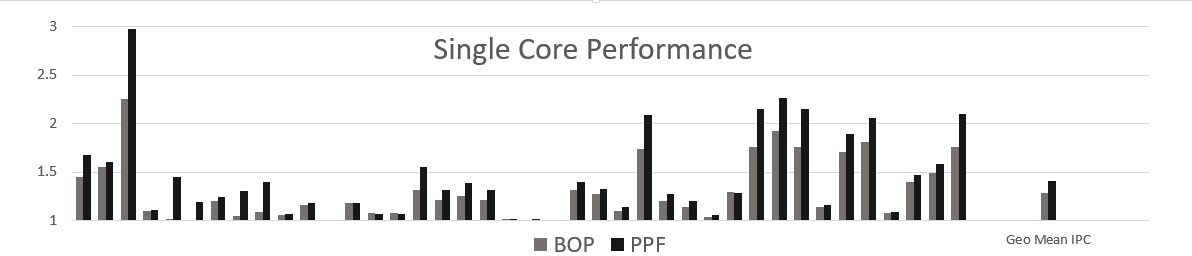
\includegraphics[width=0.85\textwidth]{Performance}
  \caption{Single Core Performance}
  \label{fig:perf}
  \end{center}
\end{figure*}



\begin{table}[h]
\begin{adjustwidth}{}{}
    \centering
    \begin{adjustbox}{width=0.72\columnwidth}
    \begin{tabular}{|c|c|c|c|}
    \hline
        \textbf{Structure} &
        \textbf{Entry} &
        \textbf{Components} &
        \textbf{Total} \\
    \hline
	\multicolumn{4}{|c|}{\textbf{L1D Prefetcher}}	\\
    \hline
	\multirow{2}{1.5cm}{Throttler}	& 	\multirow{2}{0.7 cm}{1024} &	Tag (7 bits )	&  12288	\\
					&				   &	Score (5 bits)	&  bits		\\
    \hline
	Pages Accessed			&	8			   & 	Page number (52 bits) 	& 416 bits	\\
    \hline
        \multicolumn{4}{|c|}{\textbf{Overall L1D: 12,704 bits = 1.55 KBs}}\\
    \hline
	\multicolumn{4}{|c|}{\textbf{L2C Prefetcher}}	\\
    \hline
                                            &  \multirow{5}{0.5cm}{256}    & Valid (1 bit)  &             \\
                                             &      & Tag (16 bits)        &  \multirow{2}{0.9cm}{11008}           \\
                            Signature Table  &   & Last Offset (6 bits) &  \multirow{2}{0.5cm}{bits}  \\  
                                             &      & Signature (12 bits)  &             \\
                                             &      & LRU (6 bits)         &             \\
    \hline
                                    &  \multirow{3}{0.5cm}{2048}    & $C_{sig}$ (4 bits)      &\multirow{2}{0.9cm}{98304}               \\
                       Pattern Table         &   & $C_{delta}$ (4*4 bits) &  \multirow{2}{0.5cm}{bits}  \\
                                             &      & Delta (4*7 bits)       &               \\
    \hline
        \multirow{4}{1.5cm}{Perceptron\newline}     & 4096*4    & \multirow{4}{0.8cm}{5 bits}  & \multirow{3}{1.1cm}{113280}             \\
        \multirow{3}{1.2cm}{Weights}                & 2048*2    &           &  \multirow{3}{0.5cm}{bits}  \\
                                                    & 1024*2    &           &               \\
                                                    & 128*1     &           &              \\
    \hline
        Prefetch                & \multirow{2}{0.7cm}{1024}      & \multirow{2}{1cm}{85 bits}       & 87040 \\
        Table   &           &               & bits\\
    \hline
        Reject                & \multirow{2}{0.7cm}{1024}      & \multirow{2}{1cm}{84 bits}    & 86016 \\
        Table & & & bits\\
    \hline
        \multirow{4}{1.0cm}{Global\newline\newline}   & \multirow{4}{0.2cm}{8} & Signature (12 bits)  & \multirow{4}{1.1cm}{264 bits} \\
        \multirow{3}{1.1cm}{History\newline}        &                        & Confidence (8 bits)  &                               \\
        \multirow{2}{1.2cm}{Register}               &                        & Last Offset (6 bits) &                               \\
                                                    &                        & Delta (7 bits)       &                               \\
    \hline
        Accuracy        & 1     & C$_{total}$       & 10 bits   \\
        Counters        & 1     & C$_{useful}$      & 10 bits   \\
    \hline
        \multirow{3}{1.5cm}{Global PC\newline}      &       & $PC_1$ (12 bits)      &           \\
        \multirow{2}{1.5cm}{~Trackers}              & 3     & $PC_2$ (12 bits)      & 36 bits   \\
                                                    &       & $PC_3$ (12 bits)      &           \\
    \hline
	Pages Accessed			&	8			   & 	Page number (52 bits) 	& 416 bits	\\
    \hline
        \multicolumn{4}{|c|}{\textbf{Overall L2C: 396,384 bits = 48.39 KBs}}\\
    \hline
        \multicolumn{4}{|c|}{\textbf{Total: 409,088 bits = 49.94 KBs}}\\
    \hline
    \end{tabular}
    \end{adjustbox}
    \caption{Single-core Prefetcher Hardware}
    \label{tab:PPF_overhead}
\end{adjustwidth}
\end{table}

\noindent \textbf{Single-Core Complexity:}
Table~\ref{tab:PPF_overhead}
shows a detailed analysis of the hardware overhead required to
implement the three prefetchers. It is well within the championship
budget of 64KB. In terms of L2C prefetcher's logical complexity, SPP
is a cascade of three tables, with the output of one indexing into the
next. Constructing the signature only requires simple operations like
shifting and XOR. PPF requires parallel indexing into nine different
tables and adding nine 5-bit integers, which is well within the
complexity of currently implemented perceptron-based branch
predictors.  Weight updates are done only in steps of +1 or -1.

\subsection{Multi-Core Configuration}
\label{Config-Multi}

When in a multi-core configuration, we disable the L1D Prefetcher, keep 
the same L2C Prefetcher and switch the LLC prefetcher altogether to SPP, 
without the enhanced PPF components.
We do this by leveraging the information from NUM\_CPUS parameter.
We observed that the efficient filtering mechanism in PPF helps avoid 
pollution in the shared LLC and a further attempt to do aggressive
prefetching leads to performance degradation.
Hence we re-tune SPP's thresholds towards the safer side and this
helps further boost the overall performance. 

\noindent \textbf{Multi-Core Complexity:}
Beside the single-core L2C prefetcher complexity, LLC SPP adds an overhead 
of 14.44 KBs per core, making a total of 62.83 KBs per core, which is within 
the budget allowed by the championship.
